%% Mission Objectives

%% Europa, one of the satellites of Jupiter, is probably the most
%% interesting celestial body in the Solar System due to its unique
%% characteristics, that have led some scientists to theorize a
%% scenario in which it could even be colonized in a far future. This
%% mission will therefore have the goal of better investigating the
%% surface characteristics and the potential habitability of Europa,
%% through a detailed observation of the ice-shell surface of the
%% planet and a characterization of the chemical composition of the
%% surface and the inner oceans below it. The spacecraft payload will
%% be represented by a high-resolution camera, a laser altimeter, an
%% ice-penetrating radar, a set of spectrometers and a thermal camera.

%% Top-Level Requirements
%% • Payload Mass (total): 80 kg
%% • Payload Size (total): 0.7 m x 0.7 m x 0.7 m
%% • Payload Required Power (maximum): 50 W
%% • Payload Operational Temperature Range: 150÷200 K
%% • Orbit: polar, 200 km altitude (above Europa surface)
%% • Mission Duration: at least 3 years in Europa orbit
%% • Ground Segment: ESTRACK
%% • Mission Operations Centre: ESOC
%% • Launch Date: 2020
%% • Total Mission Cost: ≤ 500 million Dollars (in FY2000 money)
%% • Mission Reliability: 0.9

\documentclass{report}
\title{AE2100 \\
  \small{Space Project 3} \\
  Europa Orbiter}
\author{Group C3 \\
  Seong Hun Lee \\
  Constantin Jux \\
  Julius Jördens \\
  Geart van Dam \\
  Tim Blondeel \\
  Aaku Kokko}
\date{}
\setcounter{secnumdepth}{-2}
\usepackage{cite}
\usepackage{hyperref}
\hypersetup{
    colorlinks=false,
    pdfborder={0 0 0},
}
\usepackage{siunitx}
\usepackage{graphicx}
\usepackage{supertabular}
\bibliographystyle{unsrt}
\newcommand{\workpkg}[1]{\part{Work Package #1}}
\newcommand{\subworkpkg}[1]{\chapter{WP #1}}
\newcommand{\deliverable}[1]{\section{D#1}}
\newcommand{\task}[1]{\subsection{Task #1}}

\begin{document}
\maketitle
\tableofcontents

\workpkg{1}

%% This Work Package deals with the mission functional analysis, the
%% definition of the spacecraft requirements and the mission profile,
%% and the initial sizing of your spacecraft.

%% WP1.1 Functional Analysis
%% WP1.2 Spacecraft Requirements
%% WP1.3 Mission Profile
%% WP1.4 Initial Sizing

%% Timeline : Weeks 1 and 2 (2-weeks total duration)

%% Deadline for Report Delivery: Monday September 17th, 12.00 hours

%% Each report shall include, as a minimum, all the Deliverables
%% listed in the sub-WP descriptions provided below (each deliverable
%% is identified by a unique code, in the form Dx.y.z). The names and
%% student numbers of the authors shall be present on the cover
%% page. The report shall also include a work division table,
%% indicating which group members have contributed to each one of the
%% tasks.

%% Deliver the printed report to the Teaching Assistant assigned to
%% your group.

\subworkpkg{1.1}

%% Tasks

%% A. Search for 5 existing (or planned) similar missions and identify
%% for these missions:

%% a. the mission objectives and, if possible, the associated mission
%% requirements;

%% b. the main elements that make up the mission and their main
%% function(s);

%% c. the main performance and design characteristics of these
%% elements.

%% B. Define the mission elements with which the design process will
%% interact (e.g.: mission operations, ground system, launch system,
%% etc.).

%% C. List the main objectives to be achieved in the design process
%% (related to, e.g., payload capability, performance, structure,
%% etc.). Mention at least 10 objectives.

%% D. For each one of the identified design objectives, list the main
%% functionalities that the design must provide in order to accomplish
%% it.

%% E. List all the design parameters that are already available (e.g.,
%% from the project description provided in Section 3) and the ones
%% which still need to be identified.

%% Deliverables

%% D1.1.1. Comparative table including all the relevant information
%% collected for the reference missions identified under Task A above.

\deliverable{1.1.1}

\begin{table}[h]
  \caption{Similar missions.}
  \begin{tabular}{p{.5\textwidth}p{.5\textwidth}}
    & \\
    & Launch date \\
    \hline
    Galileo & October 1989 \\
    Juno & August 2011 \\
    Jupiter Europa Orbiter (JEO) & February 2020 \\
    Jupiter Icy Moon Explorer (JUICE) & 2022 \\
    Cassini & October 1997 \\
  \end{tabular}
\end{table}

\begin{supertabular}{p{\textwidth}}
  The mission objectives and associated requirements \\ \hline \\

  Galileo \\
  \begin{itemize}
  \item Study Jupiter’s atmosphere, satellites, and magnetosphere by
    deploying a Jupiter orbiter and conducting various experiments.
  \item Send a probe to the surface of Jupiter to identify atmospheric
    materials and conditions that cannot be detected from outside.
  \item Venus and Earth flyby for extensive survey on the planets’
    surface and atmosphere (including imaging)
  \end{itemize}
  Requirements. Durable spacecraft and orbiter. Safe transmission of
  the data to Earth.  Strongly built probe which can survive
  penetration of the atmosphere as well as ground impact and operate
  without malfunctions. \\

  Juno \\
  \begin{itemize}
  \item Observe Jupiter's gravity and magnetic fields, atmospheric
    dynamics and composition. Thus, ultimately, investigate the
    formation and evolution of Jupiter.
  \end{itemize}

  Requirements. Durable spacecraft with maneuverability. Safe
  transmission of the data to Earth. \\

  JEO \\
  \begin{itemize}
  \item Europa’s Ocean: Characterize the extent of the ocean and its
    relation to the deeper interior
  \item Europa’s Ice Shell: Characterize the ice shell and any
    subsurface water, including their heterogeneity, and the nature of
    surface-ice-ocean exchange
  \item Europa’s Chemistry: Determine global surface compositions and
    chemistry, especially as related to habitability
  \item Europa’s Geology: Understand the formation of surface
    features, including sites of recent or current activity, and
    identify and characterize candidate sites for future in situ
    exploration
  \item Jupiter System: Understand Europa in the context of the
    Jupiter system
  \end{itemize} \\

  JUICE \\
  \begin{itemize}
  \item To characterize the conditions that may have led to the
    emergence of habitable environments among the Jovian icy
    satellites, with special emphasis on the three ocean bearing
    worlds, Ganymede, Europa, and Callisto
  \end{itemize}

  Requirements. 2 flybys of Europa, 12 flybys of Callisto. Orbit
  around Ganymede, Optimal illumination conditions and high pointing
  accuracy for high-resolution imaging. Different orbits possible. A
  minimum average downlink of 1.4Gb/day \\

  Cassini \\
  \begin{itemize}
  \item Bring the Huygens probe to Saturn’s moon Titan.
  \item Study the moons Titan and Encladus as well as the other icy
    moons
  \end{itemize} \\

  Main mission elements and their main functions \\ \hline \\

  Galileo \\ \begin{itemize}
  \item Launch (aboard a Space Shuttle). Achieve escape velocity from
    Earth and to head for Jupiter
  \item Release from the Space Shuttle and the provision of the
    thrust.
  \item Flying past the Moon, Venus and several asteroids. Carry out
    observation and imaging.
  \item Sending the probe into Jupiter's atmosphere. Identify
    atmospheric constituents and conditions that cannot be detected
    from outside.
  \item Sending the orbiter into Jovian orbit. Observe the surface,
    atmosphere, and magnetosphere of the Jupiter.
  \item Termination of the mission by plunging into Jupiter's
    atmosphere.
  \end{itemize} \\

  Juno \\ \begin{itemize}
  \item Launch (aboard a Space Shuttle). Achieve Earth escape velocity
    and head for Jupiter.
  \item Release from the Space Shuttle and the provision of thrust.
  \item Earth flyby for gravity assist.
  \item Flight to Jupiter and arrival into Jovian orbit.
  \end{itemize} \\

  JEO \\ \begin{itemize}
  \item Launch (aboard a Space Shuttle Atlas V 551). Achieve Earth
    escape velocity and head for Jupiter.
  \item Release from the Space Shuttle and the provision of thrust.
  \item Venus and Earth flyby for gravity assist.
  \item Flight to Jupiter, and Jovian orbit insertion.  insertion
  \item Transfer to Europa orbit (Europa orbit insertion) followed by
    science mapping phase.
  \item Termination of the mission. Impact the surface of Europa after
    running out of fuel.
  \end{itemize} \\

  JUICE \\ \begin{itemize}
  \item Launch by Ariana-5 ECA
  \item Cruise. Interplanetary transfer from Earth to Jupiter.
  \item Jupiter tour. A transfer to Callisto, 2 Europa and 3 Callisto
    flybys, Jupiter high latitude phase, including 9 Callisto flybys,
    and finally a transfer to Ganymede.
  \item Ganymede tour, consisting of elliptical and high altitude
    circular phases, 500km altitude orbit and a 200km altitude orbit.
  \item End of mission.
  \end{itemize} \\

  Cassini \\ \begin{itemize}
  \item Launch.
  \item Jupiter flyby to provide the final push for the trajectory to
    Saturn and to study Jupiter from two different spacecraft at the
    same time.
  \item Release of the Huygens probe to Titan.
  \item Start extended mission in which different moons of Saturn are
    studied.
  \end{itemize} \\

  Main performance and design characteristics \\ \hline \\

  Galileo \\
  \begin{itemize}
  \item Launch Vehicle. Space Shuttle Atlantis (STS-34R)
  \item The spacecraft's propulsion module consists of twelve
    10-newton (2.25-pound-force) thrusters and a single 400-newton
    (90-pound-force) engine which use monomethylhydrazine fuel and
    nitrogen-tetroxide oxidizer
  \item Spacecraft Instruments.
    \begin{itemize}
    \item Orbiter instruments. Imaging system. Near-infrared mapping
      spectrometer. Ultraviolet spectrometer.
      Photopolarimeter-radiometer. Magnetometer. Energetic-particles
      detector. Plasma detector. Plasma wave and heavy ion
      counter. Radio system
    \item Atmospheric entry probe instruments. Atmospheric structure
      instrument.  Neutral mass spectrometer. Helium abundance
      detector. Net flux
      radiometer. Nephelometer. Lightning/energetic-particles
      experiment.
    \end{itemize}
  \item Spacecraft Power. Two Radioisotope Thermoelectric Generators.
  \item Antenna Diameter. 4.8-meter.
  \end{itemize} \\

  Juno \\
  \begin{itemize}
  \item Launch Vehicle. Atlas V551
  \item Fuel Mass. 1,280 kilograms of fuel and 752 kilograms of
    oxidizer.
  \item Spacecraft Instruments. Gravity Science Experiment.
    Magnetometer, Microwave Radiometer. Particle Detector. Jovian
    Infrared Auroral Mapper (JIRAM). Ultraviolet Imaging Spectrograph
    (UVS).
  \item Spacecraft power. Solar Arrays. Dimensions of each solar array
    29.5 feet (9 meters) by 8.7 feet (2.65 meters).
  \item Propulsion. Dual mode propulsion subsystem. Bi-propellant main
    engine and mono-propellant reaction control system thrusters. The
    12 reaction control system thrusters allow translation and
    rotation about three axes.
  \item Command and Data Handling. A RAD750 flight processor with 256
    megabytes of flash memory and 128 megabytes of DRAM local
    memory. Provides 100 Mbps total instrument throughput.
  \item Power. Power generation is provided by three solar arrays
    consisting of 11 solar panels and one MAG boom.
  \end{itemize} \\

  JEO \\
  \begin{itemize}
  \item Launch Vehicle. Atlas V551.
  \item Radiation shielding to protect electronic components and
    assemblies.
  \item Telecommunications. 3m HGA with a 2-axis gimbal. 25 W X-band
    and Ka-band TWTAs.
  \item Attitude control. 3-axis stabilized with reaction wheels and
    coupled thrusters.
  \item Power. 540W RPS (MMRTG or ASRG). Lithium Ion battery for peak
    power management.
  \item Propulsion. Bi-propellant, 900N engine.
  \item Spacecraft instruments. Laser Altimeter (LA). Radio Science
    (RS). Ice Penetrating Radar (IPR).  VIS-IR Imaging Spectrometer
    (VIRIS).  UV Spectrometer (UVS).  Ion and Neutral Mass,
    Spectrometer (INMS).  Thermal Instrument (TI).  Narrow Angle
    Camera (NAC).  Wide Angle Camera and Medium, Angle Camera
    (WAC+MAC).  Magnetometer (MAG).  Particle and Plasma Instrument
    (PPI).
  \end{itemize} \\

  JUICE \\
  \begin{itemize}
  \item 3-axis stabilized.
  \item Power. Solar panels. 636-693W (EOM).
  \item High Gain Antenna. 3.2 m. Body fixed.
  \item X and Ka bands. Downlink > 1.4 Gbit/day.
  \item High delta-V capability (2700 m/s).
  \item Radiation level. 240krad/10 mm Al solid sphere.
  \item Dry mass at launch. ~1800kg.
  \end{itemize} \\

  Cassini \\
  \begin{itemize}
  \item 3-axis stabilized.
  \item 2,150 kg orbiter.
  \item 350kg probe.
  \item 3,132kg fuel.
  \item 3 radioisotope thermoelectric generators for 880W. 670W left
    in 2010.
  \end{itemize} \\
\end{supertabular}

\begin{table}[h]
  \caption{Sources.}
  \begin{tabular}{p{.2\textwidth}p{.8\textwidth}}
    Sources & \\ \hline & \\

    Galileo & \cite{galileonasa} and \cite{galileojpl} \\

    Juno & \cite{junonasa} \\

    JEO & \cite{jeonasa} \\

    JUICE & \cite{juiceesa} \\

    Cassini & \cite{cassininasa} \\
  \end{tabular}
\end{table}

%% D1.1.2. Block diagram showing the outcomes of Task B above (hint:
%% you can put the item to be designed in the middle, and the relevant
%% mission elements around it).

\deliverable{1.1.2}

The design will have to interact with the following mission elements.

\begin{figure}[h]
  \caption{Mission elements.}
  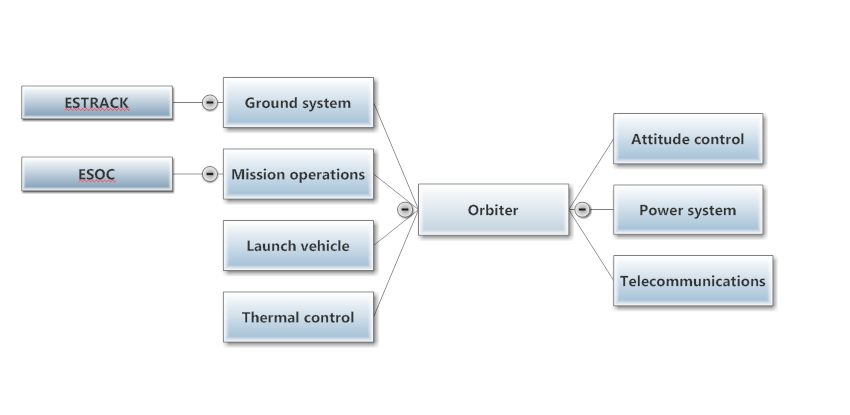
\includegraphics[width=\textwidth]{block-diagram-WP1-1B}
\end{figure}

\begin{itemize}
\item{Ground system.} The ground segment will use ESTRACK.
\item{Mission operations.} The mission operations center will be ESOC.
\item{Launch vehicle.}
\item{Thermal control.}
\item{Attitude control.}
\item{Power system.}
\item{Telecommunications.}
\item{Radiation shielding.}
\item{Propulsion systems.}
\item{S/C structures.}
\item{Orbit / trajectory}
\end{itemize}

%% D1.1.3. Numbered lists obtained from Tasks C, D and E above (note:
%% lists should be as complete as it is possible at this stage of the
%% design, and a clear justification for each listed item shall be
%% provided).

\deliverable{1.1.3}

The following mission objectives must be met

\begin{enumerate}
\item{Payload size.} 0.7m x 0.7m x 0.7m
\item{Payload orientation.} Free View for Camera, etc.
\item{$\Delta$-V budget.} To be determined.
\item{Power requirements.} Maximum payload power: 50W
\item{Payload operational temperature.} 150--200K
\item{Lifetime.} More than 3 years.
\item{Data storage and transfer.} To be determined.
\item{Reliability.} At least 0.9.
\item{Shielding (radioactive radiation).} To be determined.
\end{enumerate}

The already known design parameters are

\begin{enumerate}
\item{Payload mass.} 80kg
\item{Payload dimensions.} 0.7m x 0.7m x 0.7m
\item{Payload required power.} 50W
\item{Payload operational temperature range.} 150--200K
\item{Orbit.} Polar, 200km above Europa surface.
\item{Mission duration.} At least 3 years in Europa orbit.
\item{Launch date.} Around 2020
\item{Total mission cost.} Less than 500 million FY2000 USD.
\item{Mission reliability.} 0.9
\end{enumerate}

The design parameters yet to be determined include

\begin{enumerate}
\item{Radiation environment and shielding.} Radiation levels demand adequate
  shielding.
\item{$\Delta V$-budget.}
\item{Payload orientation.} Free field of view for instruments.
\item{Data storage and transfer.}
\end{enumerate}

\subworkpkg{1.2}

%% Tasks

%% A. Familiarize with the celestial body object of the mission (Moon,
%% Mars or Europa) and collect all the relevant information on it
%% (e.g., gravitation coefficient, radius, atmospheric density,
%% orbital period, eclipse periods, solar intensity received, albedo,
%% etc.).

%% B. Search for at least 5 existing (or planned) spacecrafts to be
%% used as a reference for your design, i.e.  for which the S/C
%% specifications and characteristics are similar to the ones expected
%% in your mission.  Collect information on the design of the
%% identified reference spacecrafts (e.g., mass and power budgets,
%% size, structure configuration, payload characteristics, orbital
%% parameters, etc.).

%% C. List a detailed set of requirements for your design, taking into
%% account the top-level mission requirements (from the project
%% description provided in Section 3) and the characteristics of the
%% identified reference spacecrafts. Remember: the requirements shall
%% be SMART (Specific, Measurable, Achievable, Realistic,
%% Time-bound)!! Whereas possible express them as numbers, preferably
%% in the form of a range of values.

%% D. From the complete list of requirements, identify at least 10
%% driving requirements for your design, i.e.  requirements that will
%% play a major role in the design process. Provide an adequate
%% justification for your choice.

%% Deliverables

%% D1.2.1. Table including all the relevant data on the celestial body
%% object of the mission.

\deliverable{1.2.1}

Table including all the relevant data on the celestial body object of
the mission.  Data is from
\cite{nasaeuropa,Jupiter,Europa,Europa2,Europa3}.

\begin{itemize}
\item{Orbit Size Around Jupiter (semi-major axis):} \SI{671,100}{km}
\item{Periapsis (closest):} \SI{664,792}{km}
\item{Apoapsis (farthest):} \SI{677,408}{km}
\item{Sidereal Orbit Period (Length of Year):} 3.551181041 Earth days
\item{Orbit Circumference:} \SI{4216552.51}{km}
\item{Average Orbit Velocity:} \SI{49476.1}{km/h}
\item{Orbit Eccentricity:} 0.0094
\item{Orbit Inclination:} \ang{0.466}
\item{Mean Radius:} \SI{1560.8}{km}
\item{Equatorial Circumference:} \SI{9806.8}{km}
\item{Volume:} \SI{15926867918}{km^3}
\item{Mass:} \SI{47998438387492700000000}{kg}
\item{Planet density:} \SI{3.013}{g/cm^3}
\item{Surface Area:} \SI{30612893.23}{km^2}
\item{Surface Gravity:} \SI{1.315}{m/s^2}
\item{Escape Velocity:} \SI{7293}{km/h}. Scientific Notation: \SI{2026}{m/s}
\item{Sidereal Rotation Period (Length of Day):} 3.551 Earth days
\item{Atmospheric Constituents:} Oxygen
\item{Temperature:} \SI{102}{K}
\item{Albedo:} 0.67
\item{Solar intensity:} \SI{49.8}{W/m^2}
\end{itemize}

%% D1.2.2. Comparative table including all the relevant design data
%% collected for the reference spacecrafts identified under Task B
%% above.

\deliverable{1.2.2}

Comparative table including all relevant data of reference
spacecrafts.

\begin{longtable}{lp{.8\textwidth}}
  \caption{Reference spacecraft data.} \\ \toprule

  \multicolumn{2}{c}{Launch vehicle} \\ \midrule

  Galileo & Space Shuttle Atlantis (STS-34R) \\

  Juno & Atlas V551 (Atlas first stage with five solid rocket
  boosters, Centaur upper stage) \\

  JEO & \\

  JUICE & \\

  Cassini & Titan IV-B/Centaur launch vehicle \\

  \multicolumn{2}{c}{Mass} \\ \midrule

  Galileo & Orbiter: \SI{2223}{kg} Probe: \SI{339}{kg} \\

  Juno & \SI{3625}{kg} total at launch, consisting of \SI{1593}{kg} of
  spacecraft, \SI{1280}{kg} of fuel and \SI{752}{kg} of oxidizer \\

  JEO & Launch Mass Capability, \SI{5040}{kg} Launch Vehicle Adapter,
  \SI{123}{kg} Flight System, \SI{1367}{kg} Propellant (for
  \SI{2260}{m/s}), \SI{2646}{kg} Remaining usable launch mass,
  \SI{973}{kg} (for contingency and system margin) \\

  JUICE & Dry mass at launch: ~\SI{1800}{kg}. Chemical propellant:
  \SI{3000}{kg}. Payload mass: \SI{104}{kg} \\

  Cassini & Spacecraft \SI{2442}{kg}. Propellant \SI{3132}{kg}. Total
  Mass \SI{5574}{kg}. Orbiter Weight: \SI{5712}{kg} with fuel, Huygens
  probe, adapter, etc. \SI{2125}{kg} unfueled orbiter alone \\

  \multicolumn{2}{c}{Dimensions} \\ \midrule

  Galileo & Orbiter: 6.15 meters Probe: 86 cm \\

  Juno & 3.5 meters high, 3.5 meters in diameter \\

  JEO & \\

  JUICE & \\

  Cassini & Orbiter dimension: 6.7 meters high; 4 meters wide \\

  \multicolumn{2}{c}{Power} \\ \midrule

  Galileo & Two Radio\-isotope Thermoelectric Generators. Max power:
  \SI{570}{W} \\

  Juno & Solar Arrays: length of each solar array \SI{9}{m} by
  \SI{2.65}{m} Total surface area of solar arrays: more than
  \SI{60}{m^2} \\

  JEO & \SI{540}{W} RPS (MMRTG or ASRG) Lithium Ion battery for peak
  power management \\

  Juice & Power: solar panels: \SI{636}{W}--\SI{693}{W} (EOM). Solar array
  \SI{60}{m^2}--\SI{75}{m^2} \\

  Cassini & 885 watts (633 watts at end of mission) from radioisotope
  thermoelectric generators \\

  \multicolumn{2}{c}{Propulsion} \\ \midrule

  Galileo & The spacecraft's propulsion module consists of twelve
  10-newton (2.25 pound\--force) thrusters and a single 400-newton
  (90-pound-force) engine which use monomethylhydrazine fuel and
  nitrogen-tetroxide oxidizer \\

  Juno & Dual mode propulsion subsystem; a bi-propellant main engine and
  mono-propellant reaction control system thrusters. The 12 reaction
  control system thrusters allow translation and rotation about three
  axes \\

  JEO & Bi-propellant , \SI{900}{N} gimbaled engine \\

  JUICE & High delta-V capability (2700 m/s) \\

  Cassini & Two engines, 445 Newton thrust each \\

  \multicolumn{2}{c}{Antenna diameter} \\ \midrule

  Galileo & 4.8-meter \\

  Juno & 4 meter \\

  JEO & \\

  JIME & 3m \\

  Cassini & 4m \\

  \multicolumn{2}{c}{Total cost} \\ \midrule

  Galileo & \$1.3 billion \\

  Juno & \$1.1 billion \\

  JEO & \\

  JIME & \\

  Cassini & \$3.27 billion \\

  \multicolumn{2}{c}{Additional characteristics} \\ \midrule

  Galileo & \\

  Juno & \\

  JEO & \SI{3}{m} HGA with 2-axis gimbal, \SI{25}{W} X-band and
  Ka-band TWTAs \\

  JIME & X and Ka bands, Downlink 1.4 Gbit/day \\

  Cassini & \\ \bottomrule
\end{longtable}

Sources used
\cite{Galileo,Galileo2,Juno,JEO,Juice,Juice2,Cassini,Cassini2}.

%% D1.2.3. Detailed list of design requirements, with a clear
%% indication of the driving requirements.

\deliverable{1.2.3}

Design Requirements
\begin{itemize}

\item{Propulsion}
  \begin{itemize}
  \item{The spacecraft should be able to generate enough thrust in
    order to get in the flight path to Jupiter after being separated
    from the launcher}
  \item{The propulsion should be provided in such a way that direction
    of the flight path can be controlled}
  \item{The spacecraft should be able to provide propulsion which can
    create the desired $\Delta V$ in order to achieve interplanetary
    transfer (Earth -- Jupiter \& Jupiter -- Europa)}
  \item{The propulsion should be provided in case of undesired
    de-orbiting}
  \end{itemize}

\item{Power}
  \begin{itemize}
  \item{At least 50 watts of power should be provided for the payload
    (spacecraft instruments), which will be gained from the solar
    arrays (during exposure to sunlight) and batteries (during
    eclipse)}
  \end{itemize}

\item{Structural Performance}
  \begin{itemize}
  \item{The spacecraft structure should be able to endure the loads
    that are expected to occur during the launch}
  \item{The spacecraft structure should be able to endure the pressure
    difference that is expected to occur during the missions}
  \item{Natural frequency of the spacecraft should be avoided during
    the missions}
  \end{itemize}

\item{Endurance and structural integrity}
  \begin{itemize}
  \item{The spacecraft should resist fatigue and environmental
    deterioration at least over 3 years}
  \item{Reliability should be higher than 0.3}
  \end{itemize}

\item{Data Collection}
  \begin{itemize}
  \item{The spacecraft payload should be able to fully deploy the
    implemented instruments, such as high-resolution camera, laser
    altimeter, ice-penetrating radar, spectrometers, and thermal
    camera}
  \item{Data should be collected and stored securely in the spacecraft
    until the transmission to the ground station}
  \end{itemize}

\item{Communication}
  \begin{itemize}
  \item{Transmission rate should be high enough so that stored data
    can be transmitted properly without being overloaded and/or lost:
    the antenna should have gain that is high enough, and diameter
    that is large enough}
  \end{itemize}

\item{Attitude control and stability}
  \begin{itemize}
  \item{The spacecraft should be able to rotate around all 3-axes to
    control its attitude and point to desired direction}
  \end{itemize}

\item{Thermal control}
  \begin{itemize}
  \item{The spacecraft needs to have required absorptivity and
    emissivity level to achieve a heat balance at
    \SI{150}{K}--\SI{200}{K}}
  \end{itemize}

\end{itemize}

Ten driving requirements:
\begin{enumerate}
\item{The spacecraft should be able to generate enough thrust in order
  to get on the flight path to Jupiter after being separated from the
  launcher:} This is one of the factors that determine the amount of
  fuel and type of main engine/thruster for the spacecraft.
\item{The propulsion should be provided in such a way that the
  direction of the flight path can be controlled:} This
  (maneuverability)has to be taken into account when considering the
  location of the thruster(s).
\item{The spacecraft should have sufficient propulsion in order to
  provide the desired delta-V necessary to achieve interplanetary
  transfer (Earth -- Jupiter \& Jupiter -- Europa):} This should be
  considered when determining the propellant mass.
\item{At least \SI{50}{W} of power should be provided for the payload
  (spacecraft instruments), which will be delivered by the solar
  arrays during exposure to sunlight and batteries during eclipse:}
  This should be considered when determining the size and type of the
  solar array as well as the batteries.
\item{The spacecraft structure should be able to endure the pressure
  difference that is expected to occur during the mission:} This will
  determine the load-bearing structure of the spacecraft.
\item{Reliability should be higher than 0.9:} The reliability of
  subsystems should be considered and selected accordingly.
\item{The spacecraft payload should be able to fully deploy the
  included instruments, such as the high-resolution camera, laser
  altimeter, ice-penetrating radar, spectrometers, and the thermal
  camera:} This will determine the design of the payload and its
  relative location within the spacecraft.
\item{The transmission rate should be high enough so that stored data
  can be transmitted properly without being overloaded and/or lost:
  the antenna should have gain that is high enough, and diameter that
  is large enough:} This should be considered when determining the
  size and type of the antenna.
\item{The spacecraft should be able to rotate in all 3-axes to control
  its attitude and point to the desired direction:} This has to be
  taken into account when considering the location of the thruster(s).
\item{The spacecraft needs to have a heat balance of
  \SI{150}{K}--\SI{200}{K} and therefore requires the correct level of
  absorptivity and emissivity:} This should be considered when
  selecting the outer skin of the spacecraft.

  Sources used \cite{projectreader,fortescue2011spacecraft}.

\end{enumerate}

\subworkpkg{1.3}

%% Tasks

%% A. Using methods based on statistical data (like, for instance, the
%% ones presented in Ref. [1]), make a first vehicle level estimation
%% of the spacecraft dry mass, power, size, reliability and
%% cost. Hint: you can use the reference spacecrafts characteristics
%% found in the framework of WP 1.2 to evaluate the accuracy of the
%% methods you have adopted, or even to develop your own estimation
%% method.

%% B. Preliminarily define the orbital parameters (a, e, i, , ) and
%% the interplanetary transfer trajectory foreseen for your mission.

%% C. Estimate the total v required by the mission and, based on
%% this, the total propellant mass needed (note: this value depends on
%% the type of engines/thrusters you use!! If this has not been
%% decided yet in detail, you may still have several open options for
%% the propellant mass at this stage…). Include in your estimation all
%% the relevant mission phases (e.g. launch, transfer, orbit
%% corrections, station keeping, interplanetary transfer, etc.). Don’t
%% forget to take into account proper margins!! Hint: you can use the
%% data referred to similar missions, found in the framework of WP
%% 1.1, as a baseline for your estimation.

%% D. Choose an adequate launcher for your mission and, consequently,
%% indicate the launch location, sketch the ascent profile, estimate
%% the maximum launch loads and the required minimum longitudinal and
%% transversal natural frequencies, and identify the payload adapters
%% available for use and their characteristics.

%% E. Based on the information obtained from the previous Tasks,
%% generate a detailed mission profile and a rough timeline for the
%% mission.

%% Deliverables

%% D1.3.1. Vehicle-level estimation of the spacecraft dry mass,
%% propellant mass, power, size, reliability and cost.

\deliverable{1.3.1 Vehicle-Level Estimation}

In this section some vehicle-level estimations of the spacecraft are
given in order to identify the most important design parameters.

\subsection{Dry Mass}

For the vehicle dry mass estimation, some reference spacecrafts were
used. The dry mass of the reference spacecrafts was plotted against
the payload in the figure below.

\begin{figure}[h]
  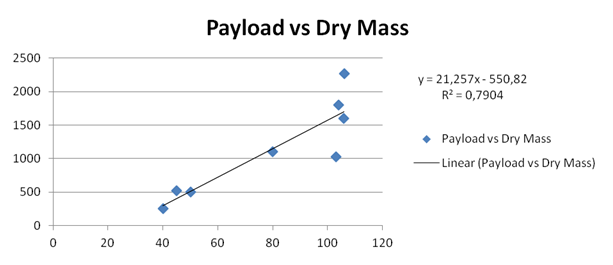
\includegraphics[width=\textwidth]{Payload-vs-DryMass}
  \caption{Payload vs. Dry Mass}
\end{figure}

The data shown in the figure above was used to estimate the dry mass
of the satelite to be designed, which was found to be \SI{1100}{kg}.

\subsection{Power}

From the reference data it can be seen that the typical used power is
between \SI{400}{W} and \SI{636}{W} with a payload of
\SI{105}{kg}. With the used payload in mind, the estimated range is
between \SI{305}{W} and \SI{485}{W}.

\subsection{Reliability}

The required reliability has to be higher than 0.9. From this
requirement the necessary failure rate can be drawn. In order to do
so, the following formula is used

\begin{equation}
  \lambda = \frac{\ln R}{t}
\end{equation}

This leads to a failure rate of 0.01317 failures per year for a
lifespan of 6.2 years.

\subsection{Initial Mass}

To calculate the total mass of the spacecraft, Tsiolkovsky's rocket
equation is used:

\begin{equation}
  \Delta V = V_e \ln \frac{M_1}{M_0}
\end{equation}

\begin{equation}
  M_0 = M_1 e^\frac{\Delta V}{V_e}
\end{equation}

The $\Delta$V has been calculated in a previous part and is found to
be \SI{2.625}{km/s}. The exhaust velocity is determined by the
specific impulse multiplied with the gravitational acceleration of
Earth. An estimated $I_{\mathrm{sp}}$ of \SI{318}{s} is used, leading to an
exhaust velocity of \SI{3117}{m/s}. Finally, an initial mass of
\SI{2550}{kg} is found. Since the calculation assumes ideal conditions
an additional margin of \SI{20}{\%} is used, leading to an estimation
of \SI{3000}{kg} for the initial mass of the spacecraft.

\subsection{Sizing}

In order to estimate the size of the spacecraft, an average mass
density of \SI{79}{kg/m^3} is used as this value was indicated in
\textit{Space Mission Engineering: The New SMAD}
\cite{Wertz2011SpaceMissionEng}. Using the following relation,

\begin{equation}
  V = \frac{M}{\rho}
\end{equation}
an estimated size of \SI{38}{m^3} is determined.

\subsection{Cost}

The cost of the spacecraft can be estimated upon the dry mass using
the following relationship\cite{AE1201CourseReader},

\begin{equation}
  C_{\mathrm{S/C}} = 0.3531 (M_{\mathrm{S/Cdry}})^{0.839}
\end{equation}
resulting in a spacecft cost of 125.8 million dollars.

%% D1.3.2. Complete mission profile (including a description of the
%% launcher requirements and characteristics) and preliminary mission
%% timeline up to EOL (End Of Life).

\deliverable{1.3.2 Complete Mission Profile}

\begin{longtable}{lp{.8\textwidth}}
  \caption{Mission Timeline.} \\

  Duration & Notes \\ \toprule

  & Launch \\

  $\le$ \SI{1}{h}

  & Launch of the spacecraft by Falcon9 into GTO \\ \toprule

  & From separation to Earth gravity assist \\

  2 years

  & This is an average time taken for Juno and Galileo spacecraft to
  go from separation to Earth gravity assist \\ \toprule

  & From Earth gravity assist to Jupiter orbit \\

  2.7 years

  & This transfer time was calculated as if Hohmann interplanetary
  transfer (elliptical orbit) was used, and the calculated value was
  double-checked with the actual transfer time for Juno and JEO
  mission; both approximately 3 years, very close to the calculated
  result.

  \begin{equation}
    T_{\mathrm{transfer}}
    =\pi\sqrt{\frac {a^3}{\mu_{\mathrm{sun}}}}
    =\pi\sqrt{\frac{(\SI{3.1}{ua})^3}{\SI{1.327d11}{km^3/s^2}}}
  \end{equation} \\ \toprule

  & Orbiting Jupiter until the departure for Europa Orbit Insertion
  \\

  4 days

  & One full orbit around Jupiter was assumed as a preparation time
  for the departure towards Europa orbit.  This is simply calculated
  as if the spacecraft is circulating in Europa's orbit, which has
  the radius of 671000km from Jupiter.

  \[ \begin{aligned}
    T_{\mathrm{orbit}}
    &= 2\pi\sqrt{\frac{a^3}{\mu_{\mathrm{jupiter}}}} \\
    &= 2\pi\sqrt{\frac
      {(\SI{671000}{km})^3}
      {\SI{126686534}{km^3/s^2}}} \\
    &= 3.6\,\mathrm{days}
  \end{aligned} \] \\ \toprule

  & Europa orbit insertion \\

  2 days

  & The target orbit around Europa has a much smaller radius of
  \SI{1760}{km} compared to the radius of Europa's orbit around
  Jupiter (\SI{671000}{km}).  Under the assumption that the Europa
  orbit insertion is done from one point of the Jovian orbit to the
  right opposite side of the orbit, the transfer time can be
  approximated as half the orbit period of Europa around Jupiter which
  would be around 2 days. \\ \bottomrule
\end{longtable}

%% D1.3.3. Graphical sketch of the spacecraft trajectory during all
%% the phases of the mission, including launch, ascent, separation,
%% parking orbit(s), interplanetary transfer and final orbit.

\deliverable{1.3.3 Spacecraft Trajectory}

The spacecraft trajectory during all mission phases has been sketched
in two parts. The first part shows a sample ascent profile of the
Falcon9 rocket, whereas the second sketch includes all transfer orbits
that will be used to reach Europa.

\begin{figure}[H]
  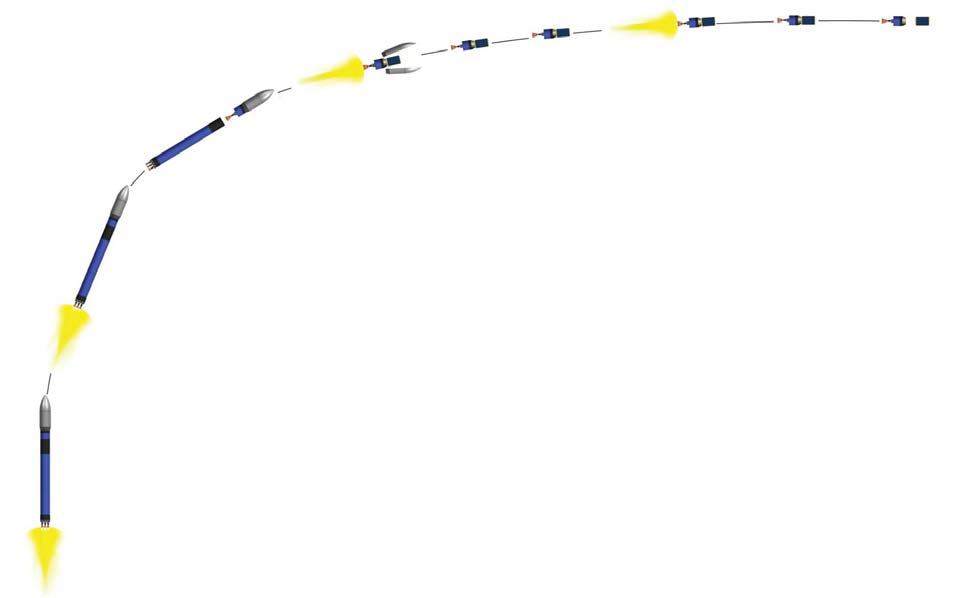
\includegraphics[width=\textwidth]{Launch-Profile}
  \caption{Sample Launch Profile: Falcon9 \cite{LVCFalcon9}}
\end{figure}

\begin{figure}[H]
  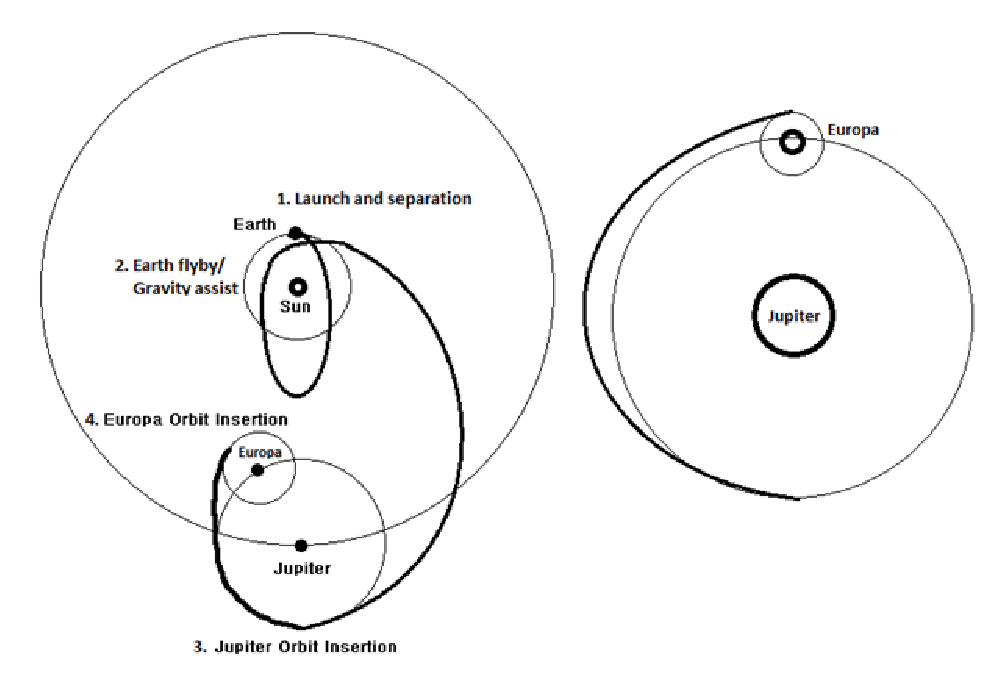
\includegraphics[width=\textwidth]{Mission-Profile}
  \caption{Complete Mission Profile}
\end{figure}

%% D1.3.4. Table showing the orbital parameters characterizing the
%% spacecraft final orbit.

\deliverable{1.3.4 Orbital Parameters}

The orbital parameters which characterize the spacecrafts final orbit
can be obtained from the table below.

\begin{longtable}{ll}
  \caption{Orbital Parameters \cite{JupiterFactSheet}} \\

  Earth-Sun distance & \SI{1}{AU} \\

  Jupiter-Sun distance & \SI{5.2}{AU} \\

  $\mathrm{\mu_{Sun}}$ & \SI{1.327d11}{km^3/s^2} \\

  $\mathrm{\mu_{Jupiter}}$ & \SI{1.267d8}{km^3/s^2} \\

  Europa-Jupiter distance & \SI{671000}{km} \\

  Europa target orbit altitude & \SI{200}{km} \\

  Europa target orbit radius & \SI{1760}{km} \\

  Semimajor axis of transfer from Earth to Jupiter

  & \SI{3.1}{AU} \\

  Eccentricity of transfer & 0.677 \\

  Inclination of transfer relative to the ecliptic plane & \ang{1;3;1}
  \\
\end{longtable}


%% D1.3.5. Estimated total v required by the mission, including a
%% table showing its breakdown into all the contributions related to
%% different mission phases and operations.

\deliverable{1.3.5 Estimated delta-V Budget}

The most traditional interplanetary transfer, the direct Hohmann
transfer orbit can be considered for this mission, since this method
has high efficiency, rapid transfer, and low radiation
exposure.\cite{Wertz2011SpaceMissionEng}

\begin{figure}[h]
  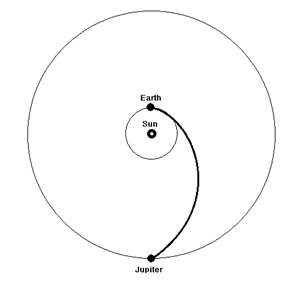
\includegraphics[width=\textwidth]{Hohmann-Orbit}
  \caption{Interplanetary Hohmann-Transfer-Orbit to Jupiter}
\end{figure}

To simplify the calculations it is assumed that both, Earth and
Jupiter, orbit the Sun in a perfectly circular orbit.  The required
orbital parameters are taken from the previous section.  Using
Hohmann-Transfer-Orbits we obtain

\begin{align*}
  \Delta V_{total} = {} &
  \Delta V_{\mathrm{perigee}}
  + \Delta V_{\mathrm{apogee}} \\
  = {} & \sqrt{\frac{\mu_{\mathrm{sun}}}{r_{\mathrm{earth}}}}
  - \sqrt{\mu_{\mathrm{sun}} \left(\frac{2}{r_{\mathrm{earth}}}
    - \frac{1}{a_{\mathrm{transfer}}}\right)} \\
  + & \sqrt{\frac{\mu_{\mathrm{sun}}}{r_{\mathrm{jupiter}}}}
  - \sqrt{\mu_{\mathrm{sun}}\left(\frac{2}{r_{\mathrm{jupiter}}}
    - \frac{1}{a_{\mathrm{transfer}}}\right)} \\
  \approx {} & \SI{8.78}{km/s} + \SI{5.63}{km/s} = \SI{14.41}{km/s} \\
\end{align*}

Given that $\Delta V_\mathrm{perigee}$ (\SI{8.78}{km/s}) is achieved
by the launcher rocket, the total $\Delta V$ that the spacecraft has
to carry itself is \SI{5.63}{km/s} which is still rather high compared
to similar existing missions, such as Juno or JUICE (See WP1.1 for
details).  Thus, it can be concluded that the Hohmann interplanetary
transfer orbit in this case does not give the most practical/optimum
trajectory for the mission.  One of the solutions to reduce the high
$\Delta V$ is to use gravity assist, which basically makes use of the
gravity of other planets during the flyby to induce a “slingshot”
effect.  Two of the existing reference missions to Jupiter use such
method to arrive at the planet Jupiter’s orbit; Galileo and Juno.  As
discussed in WP 1.1, Galileo has gravity assist of Venus-Earth-Earth,
and Juno has gravity assist of Earth.  Compared to Galileo, the Juno
spacecraft took almost 14 month less time to get to
Jupiter.\cite{SolarSystemNasa} Considering the fact that the Juno
mission shares many similar aspects with our own mission to Europa,
the mission profile of Juno can be considered as a model for our
mission.  Using one gravity assist of Earth, the orbit transfer
trajectory can be designed as shown in the figure below.

\begin{figure}[H]
  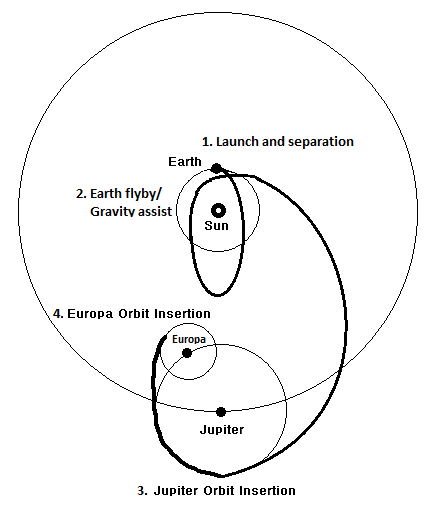
\includegraphics[width=\textwidth]{Transfer-Orbits}
  \caption{Orbit transfer trajectory using one Earth gravity assist}
\end{figure}

It should be noted that the spacecraft may temporarily orbit around
the Jupiter several times in order to achieve Europa Orbit insertion
in a favorable time and position, preferably with the minimum
$\Delta V$ and thus, the least fuel consumption. Using the data from
the Juno mission, the total $\Delta V$ budget can be estimated
\cite{DMullerNet} ($\Delta V$ for the Europa orbit insertion was taken
from the other source since the Juno mission is mainly orbiting the
planet Jupiter rather than its moon Europa). \cite{TrajectoryDesign}

\begin{longtable}{ll}
  \caption{$\Delta V$ Breakdown} \\
  Maneuver & $\Delta V$ \si{km/s} \\

  Deep space maneuver after launch until arrival at Jupiter & 733 \\

  Jupiter orbit insertion and period adjustment & 1072 \\

  Europa orbit insertion & 720 \\

  Possible orbit correction maneuver ($\Delta V$ margin) & 100 \\

  Total $\Delta V$ for spacecraft & 2625 \\
\end{longtable}

Therefore, assuming the specific impulse of \SI{318}{s} (bipropellant
system with nitrogen tetroxide/monomethylhydrazine propellants which
is the propulsion system used for Galileo --- additional remark: a
bipropellant system is also used for the Juno and the JUICE
mission)\cite{Ampac}, the required propellant mass for the spacecraft
can be calculated from the rocket equation:

\begin{equation}
  \Delta V = V_e \ln \frac{M_1}{M_0}
  = I_{\mathrm{sp}} \, g_0 \ln \frac{M_1}{M_0}
\end{equation}
\begin{equation}
  M_{\mathrm{propellant}}
  = M_0 \left( \exp \frac{\Delta V}{I_{\mathrm{sp}} \, g_0} - 1 \right)
    \approx 1.223 M_0
\end{equation}


\subworkpkg{1.4}

%% Tasks

%% A. Using methods based on statistical data and/or empirical
%% relationships (like, for instance, the ones presented in Refs. [1]
%% and [2]), define the preliminary mass and power budgets for the
%% spacecraft, i.e.  the mass and power distribution among all the
%% relevant subsystems. Pay particular attention to the definition of
%% proper design margins in your budgets.

\task{A}
Data was obtained from tables from
\cite[p. 589,590]{brown2002elements} for planetary spacecraft and
previous tasks.

The total on-orbit dry mass is

\[ m = 1100\mathrm{kg} \]

The minimum mass contingency for this class of spacecraft and stage of
design 30\%. This works out to a total on-orbit dry mass of 950kg.

Subsystem on-orbit drymass as percentages of total and absolute with
contingency margin removed are the following

\begin{center}
\begin{tabular}{rl}
Structure & $26\% \approx 290\mathrm{kg} - 86\mathrm{kg}$ \\
Thermal & $3\% \approx 33\mathrm{kg} - 9.9\mathrm{kg}$ \\
ACS & $9\% \approx 99\mathrm{kg} - 30\mathrm{kg}$ \\
Power & $19\% \approx 210\mathrm{kg} - 63\mathrm{kg}$ \\
Cabling & $7\% \approx 77\mathrm{kg} - 23\mathrm{kg}$ \\
Propulsion & $13\% \approx 140\mathrm{kg} - 43\mathrm{kg}$ \\
Telecom & $6\% \approx 66\mathrm{kg} - 20\mathrm{kg}$ \\
CDS & $6\% \approx 66\mathrm{kg} - 20\mathrm{kg}$ \\
Payload & $11\% \approx 120\mathrm{kg} - 36\mathrm{kg}$ \\
\end{tabular}
\end{center}

Total power usage is $P \approx 485{W}$.

The minimum power contingency is 90\%. Subsystem power allocation
estimates as percentages of subsystem total ($P_\mathrm{subsystems} =
P - P_\mathrm{payload} \approx 435\mathrm{W}$) and absolute with
contingency margin removed

\begin{center}
\begin{tabular}{rl}
Thermal control & $28\% \approx 120\mathrm{W} - 110\mathrm{W}$ \\
Attitude control & $20\% \approx 87\mathrm{W} - 78\mathrm{W}$ \\
Power & $10\% \approx 44\mathrm{W} - 39\mathrm{W}$ \\
CDS & $17\% \approx 74\mathrm{W} - 67\mathrm{W}$ \\
Communications & $23\% \approx 100\mathrm{W} - 90\mathrm{W}$ \\
Propulsion & $1\% \approx 4.4\mathrm{W} - 3.9\mathrm{W}$ \\
Mechanisms & $1\% \approx 4.4\mathrm{W} - 3.9\mathrm{W}$ \\
\end{tabular}
\end{center}

The launch vehicle adapter mass is given by

\[ M_{\mathrm{adapter}} = 0.0755 M_{\mathrm{launch}} + 50 \]


%% B. Based on the information gathered so far, roughly sketch at
%% least three different preliminary architectures of the spacecraft
%% with its main components (e.g. antennae, solar arrays, batteries,
%% nuclear generator, payload units, external skin). Draft at least
%% one of these preliminary sketches as a CATIA drawing.

%% C. For each one of the proposed preliminary architectures, estimate
%% the vehicle MMOI (Mass Moment of Inertia) both for the deployed and
%% un-deployed state.  Deliverables

%% D1.4.1. Tables showing the preliminary mass and power budgets for
%% the spacecraft.

\deliverable{1.4.1}

%% D1.4.2. Sketches of different optional preliminary spacecraft
%% architectures.

\deliverable{1.4.2}

%% D1.4.3. CATIA drawing of at least one preliminary spacecraft
%% architecture.

\deliverable{1.4.3}

%% D1.4.4. Estimation of the vehicle MMOI in the deployed and
%% un-deployed state.

\deliverable{1.4.4}


\workpkg{2}

%% This Work Package deals with the detailed design of the spacecraft
%% subsystems, the revision of the mass and power budgets, and the
%% definition of the final spacecraft architecture.  WP 2.1

%% Timeline : Weeks 3, 4 and 5 (3-weeks total duration)

%% Deadline for Report Delivery: Monday October 8th, 12.00 hours

%% Each report shall include, as a minimum, all the Deliverables
%% listed in the sub-WP descriptions provided below (each deliverable
%% is identified by a unique code, in the form Dx.y.z). The names and
%% student numbers of the authors shall be present on the cover
%% page. The report shall also include a work division table,
%% indicating which group members have contributed to each one of the
%% tasks.  Deliver the printed report to the Teaching Assistant
%% assigned to your group.

\subworkpkg{2.1}


%% Tasks

%% Note that all the Tasks below, related to different subsystems of
%% the spacecraft, need to be carried out in parallel, because several
%% key requirements and characteristics of the different subsystems
%% are significantly coupled each other. Hint: divide the whole group
%% into sub-groups (or individuals), each one working on a different
%% subsystem, and plan regular “system engineering meetings”
%% (e.g. daily) to exchange with the other sub-groups the information
%% related to the work done on each subsystem.

%% A. Attitude Determination and Control System (ADCS)

%% 1. Define the key subsystem requirements and functions (e.g.,
%% spacecraft stabilization and station keeping, precise orientation
%% of the payload instruments, orientation of the solar arrays, etc.).

%% 2. Evaluate whether different modes of operation of the ADCS are
%% needed or not.

%% 3. Evaluate the external and internal disturbances (forces and
%% torques) acting on the spacecraft.

%% 4. Define the type, number and size of attitude sensors and
%% attitude control actuators needed by the spacecraft (note: consider
%% sufficient redundancies!!)

%% 5. Select the sensors and actuators for the spacecraft among
%% commercially existing models, and dimension your subsystem based on
%% the characteristics of the selected components.

%% 6. Develop a block diagram that identifies the various functions
%% that need to be performed by the ADCS software.

%% B. Propulsion

%% 1. Define the key subsystem requirements and functions (e.g., orbit
%% insertion, orbital manoeuvres, interplanetary transfer,
%% etc.). Note: consider only the propulsion system on-board of the
%% orbiter spacecraft; design of optional kick stages (if any) is not
%% required.

%% 2. Define and quantify the eventual forces to be overcome by the
%% propulsion system (gravity, drag, solar radiation etc.).

%% 3. Revise your estimation for the total v required by the mission
%% and, based on it, select the thruster(s) and the propellants to be
%% used (note: decide at this stage if a “low thrust” or a “high
%% thrust” strategy has to be adopted, and select your thrusters
%% accordingly).

%% 4. Evaluate the total propellant mass needed by the mission. Don’t
%% forget to consider sufficient margins!!

%% 5. List and characterize all the components of the propulsion
%% systems; don’t consider the propellant tank(s), that will be
%% studied under the structures subsystem. If possible, select a
%% commercially available complete propulsion system.

%% 6. Generate a sketch showing the number and the location of the
%% various propulsion components in the spacecraft. Include in the
%% sketch also the major characteristics of the components shown.

%% C. Thermal Control

%% 1. Define the key subsystem requirements and functions (e.g.,
%% operational temperatures of the spacecraft components, acceptable
%% thermal gradients, etc.).

%% 2. Define the thermal environment of the spacecraft (solar
%% intensity, planet flux, albedo, etc.). Focus should be on defining
%% the thermal environments that are most critical for the design,
%% i.e. those environments that lead to max/min temperature
%% conditions.

%% 3. Estimate the internal heat generated in the spacecraft.

%% 4. Generate a straw-man subsystem design using only passive means
%% of thermal control like paints, MLI (Multi-Layer Insulation) and
%% OSR (Optical Solar Reflector).

%% 5. Using the equations provided in Ref. [1], make a first
%% estimation of the maximum and minimum equilibrium temperature of
%% both the spacecraft body and the solar array (when present), in the
%% case when no thermal control systems are used.

%% 6. Based on your equilibrium temperature estimation and on the
%% temperature requirements for the different components, define a
%% thermal control strategy for the spacecraft and select (or design)
%% the appropriate subsystem components needed for it.  Where
%% possible, use commercially existing components or materials.

%% D. Structures and Mechanisms

%% 1. Define the key requirements for the structures and mechanisms
%% subsystem.

%% 2. Define all the loads acting on the spacecraft during its
%% operations (note: take into

%% account the launch loads that you have already estimated during WP
%% 1!!). Define the safety factors to be used (you can use, for
%% instance, the values provided by the relevant ESA ECSS standards,
%% see Ref. [8]).

%% 3. Preliminarily dimension and design the primary structure of your
%% spacecraft, also choosing adequate materials for it. Based on the
%% relevant requirements for the spacecraft and its components, decide
%% if the structure has to be designed for stiffness and/or strength
%% and/or internal pressure. Hint: for your analysis you may consider
%% the primary structure to resemble a hollow cylindrical beam.

%% 4. Based on the amount of propellant(s) needed and the required
%% storage pressure, dimension and design the propellant tank(s), also
%% choosing adequate materials (note: the tank(s) can eventually be
%% used as primary structural elements!). Whereas possible, select
%% commercially existing tanks.

%% 5. Preliminarily dimension and design the supporting structure of
%% the solar arrays of your spacecraft (i.e., the mechanical structure
%% on which the array is mounted), also choosing adequate materials
%% for it. Based on the relevant requirements for the spacecraft and
%% its components, decide if the structure has to be designed for
%% stiffness and/or strength and/or internal pressure.

%% 6. Define the other mechanisms eventually needed by the spacecraft
%% (e.g. for deployment, pointing, separation, gimbal, etc.) and
%% select them among commercially existing components.

%% E. Power

%% 1. Define the key power subsystem requirements and, in particular,
%% the total amount of power required by the spacecraft during all the
%% mission phases.

%% 2. Quantify the available solar energy, i.e. the solar intensity
%% and the direction of solar radiation, the duration of day time and
%% night time (eclipse) periods, the energy received from the planet.

%% 3. Make a preliminary dimensioning of the solar arrays and, in
%% particular, a first estimation of their size (note: detailed design
%% of the solar arrays will be done during WP 3!!). You should
%% consider, for instance, whether you would like a fixed array or an
%% array that can be rotated over one or two axes to allow for ideal
%% lighting conditions.

%% 4. Based on your power requirements, evaluate the main
%% characteristic properties of the spacecraft batteries (e.g.,
%% specific energy, energy density, capacity, mass, size, etc.).

%% 5. Select the batteries and the power control components among
%% commercially existing models.

%% 6. Generate a block diagram showing the main subsystem components,
%% the power flow and the efficiencies of power conversion.

%% F. Payload

%% 1. Based on the general payload requirements and instruments list
%% provided in the project description of Section 3, choose the
%% payload components to be used by your spacecraft among commercially
%% available or previously used/proposed ones. Hint: for accomplishing
%% this task, you can also make use of the information included in
%% Ref. [7].

%% 2. Define the positioning and interface constraints for all the
%% payload components.

%% G. Other Subsystems

%% 1. For the remaining subsystems (command and data handling,
%% communications, navigation, etc.) define their key requirements and
%% functions and preliminarily select their main components. Don’t go
%% too much into the details for these subsystems; just analyse their
%% general architecture and their impact on the design of the other
%% spacecraft subsystems.

%% Deliverables

%% D2.1.1. For each one of the Tasks and sub-Tasks described above,
%% document in detail your choices, calculations and outcomes. Provide
%% detailed characteristics of the components you have chosen,
%% including their mass, size and power requirements; whereas
%% possible, include pictures and/or drawings of the components.

\deliverable{2.1.1}

\subworkpkg{2.2}

%% Tasks

%% A. Using the result obtained by WP 2.1 (in particular, the
%% requirements and characteristics of the components chosen for the
%% subsystems), define detailed mass and power budgets for the
%% spacecraft.  Clearly indicate the margins that are available.

%% B. Compare the new budgets to the preliminary ones defined in the
%% framework of WP 1, and highlight eventual changes or significant
%% differences.

%% C. Verify that the mass and power budgets are compliant to ALL the
%% mission requirements and, if necessary, re-iterate the subsystems
%% design obtained during WP 2.1.

%% Deliverables

%% D2.2.1. Tables showing the detailed mass and power budgets for the
%% spacecraft.

\deliverable{2.2.1}

\subworkpkg{2.3}

%% Tasks

%% A. Based on the operational requirements, the interfaces and the
%% dimensions of the subsystems and their components, define a
%% detailed architecture of the spacecraft including all the relevant
%% subsystems.

%% B. Draft your detailed spacecraft architecture as a CATIA drawing,
%% and compare it to the preliminary one(s) obtained in the framework
%% of WP 1.

%% Deliverables

%% D2.3.1. CATIA drawing of the spacecraft architecture. The drawing
%% shall include one or more 3D views and the necessary 2D
%% views/cut-offs needed to show the position and interfaces of all
%% subsystems.

\deliverable{2.3.1}

\workpkg{3}

%% This Work Package deals with the detailed sizing and design of an
%% important part of the power subsystem, i.e. the solar arrays.

%% Timeline : Weeks 6 and 7 (2-weeks total duration)

%% Deadline for Report Delivery: Monday October 22nd, 12.00 hours

%% Each report shall include, as a minimum, all the Deliverables
%% listed in the sub-WP descriptions provided below (each deliverable
%% is identified by a unique code, in the form Dx.y.z). The names and
%% student numbers of the authors shall be present on the cover
%% page. The report shall also include a work division table,
%% indicating which group members have contributed to each one of the
%% tasks.  Deliver the printed report to the Teaching Assistant
%% assigned to your group.

\subworkpkg{3.1}

%% Tasks

%% A. Identify at least 5 different types of solar cells that may
%% potentially be used in your spacecraft (hint: look into web sites
%% of solar cell companies like Spectrolab, Emcore, AzurSpace). For
%% each solar cell type, provide its key properties including, as a
%% minimum: power provided in peak power point, short circuit current,
%% open cell voltage, mass, efficiency, solar absorptivity and
%% emissivity, surface area per cell, performance degradation over
%% time, thermal efficiency. You should clearly indicate the
%% conditions (in particular the cell temperature) for which the
%% provided data are valid.

%% B. Make a detailed prediction of the power provided by the solar
%% arrays throughout the spacecraft lifetime. Start as a baseline from
%% the first-order estimation made during WP 2, and refine it by
%% taking into account all relevant additional effects (e.g.: solar
%% cells degradation over time, eclipse periods, variation of the
%% solar cells efficiency with temperature, batteries efficiency,
%% cable losses, possible misalignments of the solar arrays, etc.).

%% C. Define an adequate set of trade-off criteria for the selection
%% of a solar cell type, based on the identified power
%% requirements. Perform the trade-off and select the solar cell type
%% to be used in your spacecraft.

%% D. Based on the actual solar cell type selected and its specific
%% characteristics, define 3 different conceptual designs for the
%% solar arrays configuration of the spacecraft (in terms of geometry,
%% shape, size, number of cells, etc.) and draft them as CATIA
%% drawings.

%% Deliverables

%% D3.1.1. Comparative table of the identified solar cell concepts key
%% properties (including, eventually, pictures and plots).

\deliverable{3.1.1}

%% D3.1.2. Detailed calculations and plots for estimating the power
%% provided by the solar arrays during all mission phases until
%% spacecraft’s EOL.

\deliverable{3.1.2}

%% D3.1.3. Trade-off table(s) for the selection of the solar cell type
%% used in the spacecraft.

\deliverable{3.1.3}

%% D3.1.4. CATIA drawings of 3 different solar arrays configurations
%% for the spacecraft.

\deliverable{3.1.4}

\subworkpkg{3.2}

%% Tasks

%% A. Define a set of trade-off criteria and an appropriate trade-off
%% strategy for selecting one of the 3 different solar arrays
%% configurations; indicate and justify, in particular, the weight to
%% be given to each criterion.

%% B. Analyse the 3 proposed solar arrays configurations in terms of
%% at least the following aspects: total area needed to allocate the
%% required power generation; required shape, dimensions and number of
%% panels; materials, strength and stiffness; design ratios (power to
%% mass, power to area, length to width); mounting on the spacecraft
%% and orientation to the Sun.

%% C. Perform a trade-off of the 3 solar arrays configurations using
%% the criteria and weights defined in Task A above. Justify, also
%% using the results of the analysis performed for the Task B above,
%% ALL the scores given and the final configuration chosen.

%% Deliverables

%% D3.2.1. Detailed analysis of the 3 identified solar arrays
%% configurations with respect to the aspects listed in Task B above.

\deliverable{3.2.1}

%% D3.2.2. Trade-off table(s) for the selection of the solar arrays
%% configuration, including an adequate and clear explanation of all
%% the scores given.

\deliverable{3.2.2}

\subworkpkg{3.3}

%% Tasks

%% A. Determine the size and materials of the supporting structure of
%% the solar arrays and the position of the clamps between different
%% panels. Base your design on the necessity of enabling a safe launch
%% of the solar arrays structure, which translates into a requirement
%% for its eigen-frequency to be higher than 75 Hz.

%% B. Design the interfaces of the solar arrays to the rest of the
%% spacecraft. Consider in particular: the electrical interfaces; the
%% mechanisms for orienting the panels towards the Sun; the hold-downs
%% to be used during transport and launch.

%% C. Design and analyse the kinematics of the solar arrays deployment
%% and of their pointing mechanism.

%% D. Make a CATIA kinematic model of the spacecraft solar arrays.

%% Deliverables

%% D3.3.1. Complete and detailed design of: solar arrays structure;
%% interfaces to the rest of the spacecraft; deployment and pointing
%% mechanisms.

\deliverable{3.3.1}

%% D3.3.2. CATIA drawings and kinematic model of the spacecraft solar
%% arrays.

\deliverable{3.3.2}

\subworkpkg{3.4}

%% Tasks

%% A. Briefly describe the integration of the main and secondary
%% structure items of the solar arrays to the spacecraft, including
%% deployment and folding of the panel stack.

%% B. Briefly discuss the mechanical effects of the solar arrays
%% deployment process on the attitude of the spacecraft.

%% C. Describe the effects of the deployed status of the solar arrays
%% on the attitude of the spacecraft in its final orbit in relation to
%% the relevant disturbance forces as drag, solar wind, radiation
%% pressure.

%% Deliverables

%% D3.4.1. Outcomes of Tasks A, B and C above, including preliminary
%% calculations whereas necessary.

\deliverable{3.4.1}


\bibliography{ae2100}

\end{document}
